%%%%%%%%%%%%%%%%%%%%%%%%%%%%%%%%%%%%%%%%%%%%%%%%%%%%%%%%%%%%%%%%%%%%%%%%%%%%%%%%
\chapter{Реализация генератора систем инструментирования}
%%%%%%%%%%%%%%%%%%%%%%%%%%%%%%%%%%%%%%%%%%%%%%%%%%%%%%%%%%%%%%%%%%%%%%%%%%%%%%%%

В данном разделе производится постановка задач ***

***

%%%%%%%%%%%%%%%%%%%%%%%%%%%%%%%%%%%%%%%%%%%%%%%%%%%%%%%%%%%%%%%%%%%%%%%%%%%%%%%%
\section{Работа системы инструментирования}
%%%%%%%%%%%%%%%%%%%%%%%%%%%%%%%%%%%%%%%%%%%%%%%%%%%%%%%%%%%%%%%%%%%%%%%%%%%%%%%%

***
Для реализации прототипа генератора систем инструментирования был использован язык C++, возможности библиотек Boost~\cite{boost}, argparse~\cite{argparse} и tinyxml2~\cite{tinyxml2}.

%%%%%%%%%%%%%%%%%%%%%%%%%%%%%%%%%%%%%%%%
\subsection{Аннотация грамматики языка}
%%%%%%%%%%%%%%%%%%%%%%%%%%%%%%%%%%%%%%%%

***
про XML

В листинге~\ref{annotation-example} представлен пример части общей структуры файла аннотации для языка Python.

\begin{lstlisting}[frame=single, language=XML, label={annotation-example}, caption={Пример общей структуры файла аннотации}]
<!-- default pipeline: txl "%SRC%" "%TRANSFORM%" -o "%DST%" %PARAMS% -->
<annotation
  pipeline='txl "%SRC%" "%ANNOTATION_DIR%/pyindent.txl" | txl stdin "%TRANSFORM%" -o "%DST%" %PARAMS%'
  >
  <grammar ...>...</grammar>
  <lib>...</lib>
  <points-of-interest>...</points-of-interest>
  <pointcuts>...</pointcuts>
</annotation>
\end{lstlisting}

Корневой XML-элемент (тег) $annotation$ имеет опциональный атрибут $pipeline$, предназначенный для построения высокоуровневых команд обработки исходных текстов.
В случае, когда атрибут $pipeline$ не представлен в тексте аннотации, его значение становится равным команде вида <<\lstinline{txl "%SRC%" "%TRANSFORM%" -o "%DST%" %PARAMS%}>>.

В реализованном прототипе генератора систем инструментирования для построения команд обработки исходных текстов были реализованы следующие текстовые метки-заполнители (placeholder):

\begin{itemize}[noitemsep]
  \item \textit{WORKING\_DIR}   -- путь к рабочей директории процесса генератора систем инструментирования.
  \item \textit{ANNOTATON\_DIR} -- путь к директории, которая содержит файл аннотации грамматики целевого языка программирования.
  \item \textit{SRC}            -- путь к исходному файлу с текстом на целевом языке программирования; инструментируемый текст программного обеспечения.
  \item \textit{DST}            -- путь к обработанному файлу с текстом на целевом языке программирования; инструментированный текст программного обеспечения.
  \item \textit{TRANSFORM}      -- путь к файлу с описанием на языке TXL синтезированных трансформаций предоставленного исходного текста программы.
  \item \textit{PARAMS}         -- дополнительные параметры для утилиты TXL; всегда включает ***.
\end{itemize}

Кроме атрибута $pipeline$ корневой элемент содержит в себе следующие основные элементы:

\begin{itemize}[noitemsep]
  \item \textit{grammar}            -- высокоуровневое описание основных синтаксических конструкций целевого языка программирования в виде ориентированного графа (DAG).
  \item \textit{points-of-interest} -- информация, связанная с <<точками интереса>> (POI) -- выделенные пользователем пути к узлам дерева разбора, которые содержат наиболее полезные с точки зрения конечного пользователя данные, характеризующие как непосредственно точки инструментирования, так и некоторые промежуточные узлы.
  \item \textit{pointcuts}          -- информация, связанная с синтаксическими конструкциями целевого языка и точками инструментирования в них.
  \item \textit{lib}                -- дополнительные пользовательские вспомогательные TXL функции.
\end{itemize}

\nomenclature{DAG}{Directed Acyclic Graph -- ориентированный ациклический граф}
\nomenclature{POI}{Point of Interest -- точка интереса}

Далее будут более подробно рассмотрены перечисленные XML-элементы аннотации.

%%%%%%%%%%%%%%%%%%%
\subsubsection{DAG ключевых типов узлов}
%%%%%%%%%%%%%%%%%%%

Рассмотрим реализованный способ высокоуровневого описания основных синтаксических конструкций целевого языка программирования.
В листинге~\ref{annotation-dag-example} представлен пример описания взаимосвязи ключевых синтаксических конструкций для языка Java (атрибут $language$).

\begin{lstlisting}[frame=single, language=XML, label={annotation-dag-example}, caption={Пример DAG для грамматики языка Java}]
<grammar
  language="java"
  src="/grammar.txl"
  >
  <keyword-DAG>
    <package type="package_declaration">
      <imports type="repeat import_declaration"/>
      <class type="class_declaration">
        <body type="class_or_interface_body">
          <method type="method_declaration">
            <if type="if_statement">
              <else type="else_clause"/>
            </if>
            <switch type="switch_statement">
              <case type="switch_alternative"/>
            </switch>
            <for type="for_statement"/>
            <while type="while_statement"/>
            <do_while type="do_statement"/>
            ...
          </method>
        </body>
      </class>
    </package>
  </keyword-DAG>
</grammar>
\end{lstlisting}

В разработаном прототипе генератора систем инструментирования иерархические взаимосвязи между основными синтаксическими конструкциями и понятиями целевого языка программирования описываются в виде ориентированного ациклического графа (в данном случае -- дерева), вложенного в тело тега \textit{keyword-DAG} элемента $grammar$.
Имя каждого XML-элемента, вложенного в \textit{keyword-DAG} задает идентификатор синтаксической конструкции, а атрибут $type$ -- основной тип узла дерева разбора, который описывает эту синтаксическую конструкцию в соответствующей грамматике, относительный путь (относительно директории, содержащей аннотацию) к TXL-файлу которой задается с помощью атрибута $src$ основного элемента $grammar$.
Основной тип узла используется при построении раличных TXL функций для фильтрации.
Описание остальных характеристик ключевых конструкций производится при объявлении существующих точек инструментирования.
Такое разделение было выплнено с учетом ручного составления файла аннотации, вследствие чего, содержимое тега \textit{keyword-DAG} играет роль однозначного отображения идентификаторов ключевых синтаксических конструкций в типы узлов грамматики целевого языка программирования.

%%%%%%%%%%%%%%%%%%%
\subsubsection{Описание POI}
%%%%%%%%%%%%%%%%%%%

В листинге~\ref{annotation-pois-example} приведен фрагмент аннотации для языка Java, в котором описываются несколько <<точек интереса>>, такие как (атрибут $id$) <<class\_name>>, <<method\_name>> и <<if\_condition>>.

\begin{lstlisting}[frame=single, language=XML, label={annotation-pois-example}, caption={Пример}]
<points-of-interest>
...
  <point
    id="class_name"
    keyword="class"
    value-of="class_header:class_name"
    />

  <point
    id="method_name"
    keyword="method"
    value-of="method_declarator:method_name"
    />

  <point
    id="if_condition"
    keyword="if"
    value-of="condition"
    />
...
\end{lstlisting}

В рассмартриваемом примере точка интереса с идентификатором <<class\_name>> преобразуется в TXL функцию, исходный текст которой представлен в листинге~\ref{poi-src-example}.

\begin{lstlisting}[frame=single, language=TXL, label={poi-src-example}, caption={Пример синтезированной функции для точки интереса <<class\_name>>}]
function __POI_get___POI_CLASS_NAME kw_Class [class_declaration]
	replace [stringlit]
		_ [stringlit]
	deconstruct kw_Class
    ClassHeader0 [class_header] _ [class_body]
	deconstruct ClassHeader0
    _ [repeat modifier] 'class ClassName1 [class_name] _ [opt extends_clause] _ [opt implements_clause]
	construct ClassName1_str [stringlit]
		_ [quote ClassName1]
	by
		ClassName1_str
end function
\end{lstlisting}

***

%%%%%%%%%%%%%%%%%%%
\subsubsection{Описание точек инструментирования}
%%%%%%%%%%%%%%%%%%%

***

\begin{lstlisting}[frame=single, language=XML, label={annotation-pointcuts-example}, caption={Пример}]
<pointcuts>
  <keyword
    name="method"
    search-type="funcdef"
    sequential="false"
    >
    <templates>
      <template kind="replace">
        'def <!--id--> <!--parameters--> ': 'INDENT <!--newline-->
          <p name="before_body"/>
          <!--repeat statement_or_newline-->
          <p name="after_body"/>
        'DEDENT
      </template>

      <template kind="match">
        'def <!--id--> <!--parameters--> ': 'INDENT <!--newline-->
          <!--repeat statement_or_newline-->
        'DEDENT
      </template>
    </templates>
    <pointcuts>
      <pointcut name="before_body" clone="if::before_body"/>

      <pointcut name="after_body">
        <paste-algorithm>
          <fragment-to-variable
            name="Additions"
            type="repeat statement_or_newline"
            each-line-postfix="Newline"
            />
          <insert-call
            function="."
            params="Additions"
            />
        </paste-algorithm>
      </pointcut>
    </pointcuts>
  </keyword>
...
\end{lstlisting}

***

\begin{lstlisting}[frame=single, language=XML, label={annotation-template-example}, caption={Пример}]
<template kind="replace">
    'def <!--id--> <!--parameters--> ': 'INDENT <!--newline-->
        <p name="before_body"/>
        <!--repeat statement_or_newline-->
        <p name="after_body"/>
    'DEDENT
</template>
\end{lstlisting}

***

\begin{lstlisting}[frame=single, language=XML, label={annotation-algo-example}, caption={Пример}]
<pointcut name="before_body" clone="if::before_body"/>

<pointcut name="after_body">
    <paste-algorithm>
        <fragment-to-variable
          name="Additions"
          type="repeat statement_or_newline"
          each-line-postfix="Newline"
          />
        <insert-call
          function="."
          params="Additions"
          />
    </paste-algorithm>
</pointcut>
\end{lstlisting}

***

Команды, доступные пользователю (составителю аннотации) при описании алгоритма инструментирования в секции $algorithm$ аннотации грамматики.

\begin{itemize}[noitemsep]
  \item \lstinline{insert-text (text)} --
  вставка текста, заданного в параметре $text$, без экранирования в точке инструментирования, а именно, в выражении секции $by$ синтезируемой функции инструментирования (I-функции).

  \item \lstinline{insert-call (function, params)} --
  вставка вызова функции с именем $function$ с параметрами $params$, разделенными символом пробела. Параметры будут вставлены как есть, что позволяет использовать ключевое слово $each$ языка TXL для работы с последовательностями (массивами и списками).

  \item \lstinline{insert-fragment ([each-line-prefix], [each-line-postfix])} --
  вставка текста фрагмента в точке инструментирования. Для каждой строки текста фрагмента опционально может быть задан некоторый текст, добавляемый в начало \textit{each-line-prefix} и в конец \textit{each-line-postfix}.

  \item \lstinline{create-variable ([name], type, value)} --
  создание TXL переменной с типом $type$, значение которой задано текстом параметра $value$. Имя переменной будет сгенерировано автоматически из названия используемого типа, но также может быть указано вручную, используя параметр $name$.

  \item \lstinline{deconstruct-variable (type, variant)} --
  добавление в функцию инструментирования (I-функцию) конструкции TXL для декомпозиции переменной с типом $type$ в соответствии с грамматикой целевого языка программирования, используя вариант с номером $variant$, если TXL тип многозначен.

  \item \lstinline{fragment-to-variable (name, type, [each-line-prefix], [each-line-postfix])} --
  создание TXL переменной в теле I-функции с типом $type$ и именем $name$, которая содержит в себе текст добавляемого фрагмента программного кода. Как и функция \textit{insert-fragment}, команда позволяет для каждой строки добавляемого текста опционально задать <<префикс>> и <<постфикс>>.
\end{itemize}

***

%%%%%%%%%%%%%%%%%%%
\subsubsection{Пользовательские функции}
%%%%%%%%%%%%%%%%%%%

***

В дополнение к перечисленному выше была реализована возможность описания пользовательских функций на языке TXL, которые необходимо добавить в выходной файл с описанием трансформаций.
В листинге~\ref{annotation-lib-example} приведен пример определенния пользователем вспомогательной функции с именем <<addToImportsIfNotExists>> (атрибут $name$).

\begin{lstlisting}[frame=single, language=XML, label={annotation-lib-example}, caption={Пример описания вспомогательной функции}]
<lib>
  <function
    name="addToImportsIfNotExists"
    apply="call"
    params="Addition:import_declaration"
    >
      <source>
        replace [repeat import_declaration]
          Imports [repeat import_declaration]
        deconstruct not * [import_declaration] Imports
          Addition
        by
          Imports [^ Addition]
      </source>
  </function>
...
\end{lstlisting}

Из приведенного примера видно, что функции задаются при помощи тега $function$, а правила -- $rule$.

Атрибут $apply$ позволяет задать один из вариантов политики исполнения данной функции/правила:
\begin{itemize}[noitemsep]
  \item <<before-all>>  -- до всех цепочек инструментирования;
  \item <<after-all>>   -- после всех цепочек инструментирования;
  \item <<call>>        -- непосредственный вызов из алгоритма работы точки инструментирования или другой функции/правила;
\end{itemize}

Атрибут $params$ позволяет задать список формальных параметров, разделенный символом <<точка с запятой>>, и их типов для функции/правила.
Как видно из листинга~\ref{annotation-lib-example}, функция <<addToImportsIfNotExists>> имеет один параметр типа <<import\_declaration>> с именем <<Addition>>.

***

%%%%%%%%%%%%%%%%%%%%%%%%%%%%%%%%%%%%%%%%
\subsection{Фрагменты программного кода}
%%%%%%%%%%%%%%%%%%%%%%%%%%%%%%%%%%%%%%%%

В листинге~\ref{fragment-example} приведен пример пользовательского параметризованного фрагмента программного кода на некотором целевом языке программирования (в данном случае -- Java).

\begin{lstlisting}[frame=single, language=XML, label={fragment-example}, caption={Пример пользовательского фрагмента}]
<fragment language="java" name="logging_message">
  <dependencies>
    <required name="logging_imports"/>
    <required name="logging_fields"/>
  </dependencies>

  <code black-list="imports" params="message">
    iLogger.log(Level.FINE, <p id="message"/>);
  </code>
</fragment>
\end{lstlisting}

Из приведенного листинга видно, что фрагмент состоит из элемента $fragment$, именуется <<logging\_message>> (атрибут $name$) и предназначается для использования при инструментировании программного кода на языке Java (атрибут $language$).
При этом фрагмент вынуждает пользователя использовать данный фрагмент с некоторыми другими фрагментами с именами <<logging\_imports>> и <<logging\_fields>> соответственно при помощи элемента $dependencies$, содержащего перечисление фрагментов, от которых зависит корректность работы добавляемого этим фрагментом программного кода.
В прототипе была реализована работа только элемента $required$, означающая строгую зависимость от включения другого фрагмента с именем, указанным в атрибуте $name$.

Для использования передаваемых параметров, перечисление которых осуществляется через запятую в атрибуте $params$ элемента $code$, в тексте фрагмента необходимо указание пустого XML-тега $p$ с атрибутом $id$, в котором указывается идентфикатор используемого параметра.
Любое вложенное содержимое тега $p$ при этом игнорируется.

%%%%%%%%%%%%%%%%%%%%%%%%%%%%%%%%%%%%%%%%
\subsection{Правила инструментирования}
%%%%%%%%%%%%%%%%%%%%%%%%%%%%%%%%%%%%%%%%

***
про язык

На рисунке~\ref{fig:layout-ruleset} приведен пример описания пользовательских правил инструментирования с помощью разработанного языка программирования с точки зрения конечного пользователя системы.

\begin{figure}[!h]
	\centering
	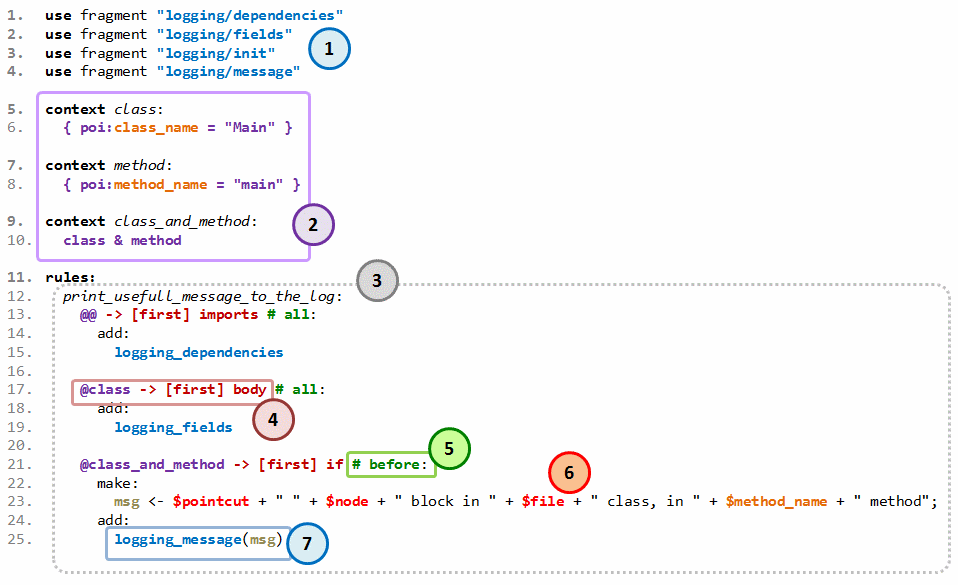
\includegraphics[width=4.2in]{layout_ruleset}
	\caption{Пример описания правил инструментирования}
	\label{fig:layout-ruleset}
\end{figure}

Основными частями пользовательского описания набора правил являются (номер пункта списка соответствует номеру на рисунке~\ref{fig:layout-ruleset}):
\begin{enumerate}[noitemsep]
  \item перечисление используемых в данном наборе правил фрагментов исходных текстов и их относительное расположение в файловой системе;
  \item перечисление интересующих пользователя контекстов инструментирования;
  \item группировка этапов инструментирования в виде именованых правил;
  \item уточнение контекста инструментирования с применением ключевых слов языка программирования и текстовых шаблонов, если таковые требуются для целей уточнения контекста согласно решаемой пользователем задачи;
  \item указание одной конкретной точки инструментирования по ее идентификатору;
  \item создание пользовательских переменных из текстовых элементов и значений констант;
  \item список имен фрагментов, вставку которых необходимо выполнить одновременно в одном и том же месте, с указанием параметров, если таковые требуются согласно тексту используемого фрагмента.
\end{enumerate}

***

Полный текст грамматики, описывающей синтаксис пользовательских правил инструментирования на языке TXL, приведен в приложении~\ref{listings:ruleset-grammar-full}.

%%%%%%%%%%%%%%%%%%%%%%%%%%%%%%%%%%%%%%%%
\subsection{Интерфейс командной строки}
%%%%%%%%%%%%%%%%%%%%%%%%%%%%%%%%%%%%%%%%

Реализованный прототип генератора систем инструментирования был реализован в виде однопоточного консольного приложения.
Для реализации интерфейса командной строки, а именно разбора параметров запуска исполнимого модуля, были использованы возможности библиотеки $argparse$~\cite{argparse}.
Данная библиотека позволяет в программном коде задавать используемые приложением параметры и одновременно с этим описывать это требование в виде текстовой пользовательской справки.

Ниже представлен список реализованных параметров запуска (в круглых скобках указано требование наличия):

\begin{itemize}[noitemsep]
  \item \lstinline{--src filenameI.lang}                -- (обязательно)
  путь к исходному файлу с текстом инструментируемого программного обеспечения, написаном на выбранном (целевом) языке программирования.

  \item \lstinline{--dst filenameO.lang}                -- (обязательно)
  путь к файлу, в котором будет сохранен инструментированный текст программы.

  \item \lstinline{--rule filename.dsl}                 -- (обязательно)
  путь к файлу, в котором описываются пользовательские правила инструметирования.

  \item \lstinline{--annotation filename.xml}           -- (обязательно)
  путь к файлу, сожержащему аннотацию к грамматике, которая содержит описание конструкций языка программирования инструментируемого программного обеспечения.

  \item \lstinline{--fragments-dir /path/to/fragments/} -- (обязательно)
  путь к директории, который необходимо считать базовым при поиске используемых пользователем при описании правил инструментирования фрагментов текста на целевом языке программирования.

  \item \lstinline{--disable "rule_name_1;rule_name_2"} -- (опционально)
  разделенный символом <<точка с запятой>> список названий пользовательских правил инструментирования, которые необходимо игнорировать при синтезе описания трансформаций для утилиты TXL.

  \item \lstinline{--no-cache}         -- (опционально)
  игнорировать ранее сохраненные результаты синтеза пользовательского набора правил, если таковые имеются.

  \item \lstinline{--txl-params}       -- (опционально)
  дополнительные параметры для утилиты TXL, передаваемые на завершающем этапе -- при выполнении трансформаций.

  \item \lstinline{--scis-grm-ruleset} -- (обязательно)
  путь к грамматике, которая на языке TXL описывает структуру файлов с пользовательскими правилами инструментирования.
  \item \lstinline{--scis-grm-txl}     -- (обязательно)
  путь к грамматике, которая на языке TXL описывает сам язык TXL.
\end{itemize}

Параметры \lstinline{--scis-grm-ruleset} и \lstinline{--scis-grm-txl} используются для сокращения числа обращений к файловой системе в случае, если бы значения, задаваемые в этих параметрах, хранились бы в файлах настройки разработанного прототипа генератора систем инструментирования.

%%%%%%%%%%%%%%%%%%%%%%%%%%%%%%%%%%%%%%%%
\subsection{Выходные артефакты генератора}
%%%%%%%%%%%%%%%%%%%%%%%%%%%%%%%%%%%%%%%%

***
про кэш и откат/копирование при ошибках

Для вычисления хэш-суммы был использован алгоритм криптографического хэширования SHA-1, представленный в бибилотеке Boost как дополнительный компонент, используемый обычно при генерации UUID-номера.
В качестве альтернативы также доступен альгоритм MD5, однако он имеет меньшую длину результирующей последовательности бит (128 против 160 у SHA-1).

\nomenclature{UUID}{Universal Unique IDentifier -- универсальный уникальный идентификатор}
\nomenclature{SHA-1}{Secure Hash Algorithm 1 -- 160-битный алгоритм криптографического хэширования}
\nomenclature{MD5}{Message Digest 5 -- 128-битный алгоритм хэширования}

%%%%%%%%%%%%%%%%%%%%%%%%%%%%%%%%%%%%%%%%
\subsection{Обработка исключительных ситуаций}
%%%%%%%%%%%%%%%%%%%%%%%%%%%%%%%%%%%%%%%%

Помимо копирования файла с исходным текстом в качестве инструментированного, как было запланировано на этапе проектирования, для упрощения навигации пользователя в случаях наличия семантических ошибок в тексте описания пользовательских правил инструментирования в грамматику, при помощи которой выполняется разбор этого описания, были добавлены нетерминальные символы $srclinenumber$, которые позволяют сохранять номер строки в анализируемом тексте.
Номера строк выводятся в некоторых (в зависимости от контекста и доступности информации о номере строки) сообщениях об ошибоках.
Неполная доступность информации о номере строки обосновывается тем, что данная функциональность была добавлена исключительно в демонстрационных целях.

%%%%%%%%%%%%%%%%%%%%%%%%%%%%%%%%%%%%%%%%%%%%%%%%%%%%%%%%%%%%%%%%%%%%%%%%%%%%%%%%
\section{Синтез цепочек TXL функций}
%%%%%%%%%%%%%%%%%%%%%%%%%%%%%%%%%%%%%%%%%%%%%%%%%%%%%%%%%%%%%%%%%%%%%%%%%%%%%%%%

***

Построение TXL функций выполняется в соответствии со следующим алгоритмом:
\begin{enumerate}[noitemsep]
  \item загрузка, разбор и проверка зависимостей указанных фрагментов программного кода в соответствии с предоставленным описанием правил инструментирования;
  \item расчет максимальных растояний для каждого узла направленного ациклического графа ключевых конструкций целевого языка программирования в соответствии с предоставленной аннотацией грамматики;
  \item построение оберток над стандартными \textit{текстовыми} операциями сравнения (W-функции);
  \item построение функций для реализации функциональности точек интереса (G-функции);
  \item построение функций проверки принадлежности узлов CST контекстам инструментирования;
  \item построение цепочек функций в соответствии с правилами инструментирования с учетом значения аргумента командной строки \lstinline{--disable};
  \item построение вспомогательных TXL функций;
  \item построение дополнительных пользовательских функций и правил, взятых из секции $lib$ аннотации грамматики;
  \item построение главной TXL функции <<main>> и применение политик использования дополнительных пользовательских функций;
\end{enumerate}

***

Цепочки вызовов функций запускаются посредством прямого вызова первых функций в каждой из функции главной функции с именем <<main>>, где  основным параметром всегда является корневой элемент конкретного дерева разбора с типом $program$.
Результаты работы первой цепочки функций передаются далее одна за другой.

В листинге~\ref{main-example} приведен пример исходного текста функции <<main>>.
Символ <<...>> содержат имена функций, которые были сокращены для повышения удобочитаемости.

\begin{lstlisting}[frame=single, language=TXL, label={main-example}, caption={Пример исходного текста главной функции}]
function main
	replace [program]
		Program [program]
	by
		Program
		[..._refiner_imports_first0]
		[..._refiner_class_level0__helper]
		[..._collector_class_and_method_m_633_uid5]
		[..._collector_class_and_method_m_633_uid8]
		[simplify]
end function
\end{lstlisting}

Связывание нескольких TXL функций в единую последовательность было реализовано посредством наследования предметно-ориентированных типов функций от класса <<CallChainElement>>, описание которого приведено в листинге~\ref{chain-element-sample}.

\begin{lstlisting}[frame=single, language=C, label={chain-element-sample}, caption={Исходный код определения элемента цепочки вызовов}]
struct CallChainElement {
  /// calleR
  TXLFunction const* callFrom = nullptr;
  /// calleE
  TXLFunction const* callTo = nullptr;
}; // CallChainElement
\end{lstlisting}

***

Ниже представлена общая структура цепочки вызовов программно-синтезируемых предметно-ориентированных функций:
\begin{enumerate}[noitemsep]
  \item C-функции -- функции сбора информации.
  \item F-функции -- функции фильтрации.
  \item R-функций -- функций уточнения контекста.
  \item I-функции -- функции инструментирования.
\end{enumerate}

Кроме этого используются следующие вспомогательные автоматически-синтезируемые TXL функции:
\begin{itemize}
  \item G-функции -- функции получения узлов, содержащих полезные значения (так называемых \textit{точек интереса}), из промежуточных узлов дерева разбора, имеющих TXL тип, который описывает какую-либо важную синтаксическую конструкцию целевого языка программирования.
  \item H-функции -- функции проверки принадлежности определенному контексту по передаваемым параметрам.
  \item W-функции -- функции-обертки стандартных операторов сравнения и поиска, выполняемых над текстовыми данными.
\end{itemize}

***

%%%%%%%%%%%%%%%%%%%%%%%%%%%%%%%%%%%%%%%%
\subsection{Функции сбора информации}
%%%%%%%%%%%%%%%%%%%%%%%%%%%%%%%%%%%%%%%%

***

C-функции (англ. $collect$) -- это TXL функции, специализированные по типу обрабатывамых узлов дерева разбора, предназначенные для накопления информации из узлов древа разбора, которая впоследствии используется для определения, соответствует-ли рассматриваемый/обрабатываемый конечный узел дерева разбора выбранному контексту инструментирования.

Принцип работы таких функций заключается в вызове следующей функции из цепочки с передачей ей всех значений аргументов, которые были получены текущей, и текущего рассматриваемого узла, тип которого содержит необходимые сведения для дальнейших операций, таких как определение соответствия контексту и формирование значений для пользовательских переменных, используемых при заполнении исользуемого фрагмента исходного кода.

C-функции опираются на специфику работы функций-правил~(rule) языка TXL: правилу $R_{(T,P)}$ будут даны на рассмотрение все узлы текущего под-дерева $G_{sub}$, соответствующие заявленому типу $T$ и сопоставимые шаблону $P$.

В листинге~\ref{cfunc-example} приведен пример исходного TXL кода простой C-функции с именем \lstinline{CollectorFuncB}, которая получает в виде аргумента некоторый узел с типом \lstinline{class_declaration}, выполняет копирование обрабатываемого узла с типом \lstinline{method_declaration} и передает эти данные (два узла, переданный в аргументах и обрабатываемый) следующей функции по цепочке вызовов с именем \lstinline{CollectorFuncC}.

\begin{lstlisting}[frame=single, language=TXL, label={cfunc-example}, caption={Пример C-функции}]
rule CollectorFuncB kw_Class [class_declaration]
  skipping [method_declaration]
  replace $ [method_declaration]
    __NODE__ [method_declaration]
  by
    __NODE__ [CollectorFuncC kw_Class __NODE__]
end rule
\end{lstlisting}

Стоит отметить, что существуют разные подходы к решению задачи передачи информации по цепочке функций:
\begin {itemize}[noitemsep]
  \item аргументы функций
    \begin{itemize}[noitemsep]
      \item добавление новых аргументов в конец (слева-направо)
      \item добавление новых аргументов в начало (справа-налево)
    \end{itemize}
  \item глобальные переменные
  \item использование средств ввода-вывода среды TXL для временного хранения результатов во внешнем, родительском для утилиты TXL, процессе
\end{itemize}

Как видно из приведенного примера, для реализации прототипа был выбран первый способ передачи данных о необходимых узлах дерева разбора-- посредством аргументов функций, где новые узлы добавляются в конец.

***

Ограничения описанного выше способа организации сбора информации об узлах дерева разбора, примененного в разработанном прототипе генератора систем инструментирования:
\begin{itemize}[noitemsep]
  \item Синтаксическое дерево исходного текста программы не содержит циклов по типам узлов -- при спуске от корня к листьям каждый \textit{сохраняемый} тип узла встречается не более одного раза
  \item ???
\end{itemize}

***

%%%%%%%%%%%%%%%%%%%%%%%%%%%%%%%%%%%%%%%%
\subsection{Функции фильтрации по контексту}
%%%%%%%%%%%%%%%%%%%%%%%%%%%%%%%%%%%%%%%%

***

F-функции (англ. $filter$) -- это TXL функции, специализированные по типу обрабатывамых узлов дерева разбора, предназначенные для фильтрации узлов CST дерева разбора относительно описываемых конечным пользователем контекстов инструментирования.

В листинге~\ref{ffunc-example} приведен пример F-функции.

\begin{lstlisting}[language=TXL, label={ffunc-example}, caption={Пример F-функции}]
function filteringFunction kw_Class [class_declaration] kw_Method [class_declaration]
  skipping [method_declaration]
  replace $ [method_declaration]
    __NODE__ [method_declaration]
  construct __VOID__ [any]
    % void
  where
    __VOID__ [belongs_to_class_and_method kw_Class kw_Method]
  by
    __NODE__ [refinerFunction kw_Class kw_Method]
end function
\end{lstlisting}

***

%%%%%%%%%%%%%%%%%%%%%%%%%%%%%%%%%%%%%%%%
\subsection{Функции уточнения контекста}
%%%%%%%%%%%%%%%%%%%%%%%%%%%%%%%%%%%%%%%%

После проверки контекста функцией-фильтром, производится вызов первой функции из последовательности R-функций.

R-функции (англ. $refine$) -- это TXL функции, специализированные по типу обрабатывамых узлов дерева разбора, предназначенные для уточнения контекста...

В листинге~\ref{rfunc-example} приведен пример R-функции.

\begin{lstlisting}[frame=single, language=TXL, label={rfunc-example}, caption={Пример R-функции}]
function refinerFunction kw_Class [class_declaration] kw_Method [class_declaration]
  replace * [repeat declaration_or_statement]
    __NODE__ [if_statement] __TAIL__ [repeat declaration_or_statement]
  construct __SINGLE_BOX_ARRAY__ [repeat declaration_or_statement]
    __NODE__ % +empty
  construct __PROCESSED__ [repeat declaration_or_statement]
    __SINGLE_BOX_ARRAY__ [instrumentationFunction kw_Class kw_Method]
  by
    __PROCESSED__ [. __TAIL__]
end function
\end{lstlisting}

***

Вид и структуру порождаемой R-функции определяет используемый модицикатор, указываемый пользователем при составлении правил инструментирования.
Были реализованы следующие модификаторы для уточняющих функций:

\begin{itemize}[noitemsep]
  \item \underline{first} -- поиск и обработка только самого \textit{первого} встреченного узла из текущего поддерева разбора в соответствии с типом, заданным в аннотации грамматики при описании синтаксической конструкции целевого языка программирования;
  \item \underline{all}   -- поиск и обработка \textit{всех узлов} в соответствии с типом, заданным в аннотации грамматики при описании синтаксической конструкции целевого языка программирования;
  \item \underline{level} -- поиск и обработка узлов, находящихся на \textit{одном уровне} (первом) вложенности таких узлов друг в друга.
\end{itemize}

На рисунках \ref{fig:modifier_level_a} и \ref{fig:modifier_level_b} показаны обобщенные примеры, демонстрирующие оказываемое модификатором <<level>> влиянние на поведение уточняющей функции.
Красным цветом выделены <<целевые>> объекты, тип которых требуется обработать.
Жирным выделены номера только тех объектов, которые соответствуют выражению <<\textit{первый уровень вложенности красных объектов друг в друга}>>.

\begin{figure}[!h]
	\centering
	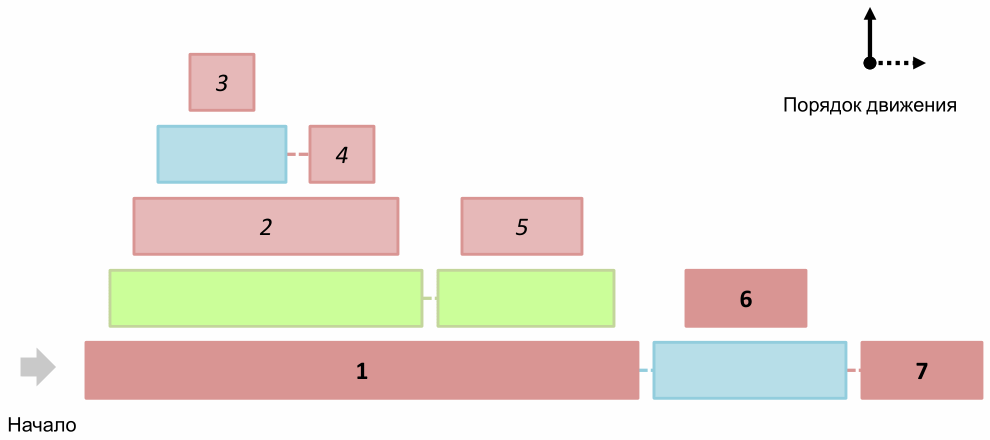
\includegraphics[width=3.2in]{modifier_level_a}
	\caption{Пример применения модификатора <<level>>.}
	\label{fig:modifier_level_a}
\end{figure}

\begin{figure}[!h]
	\centering
	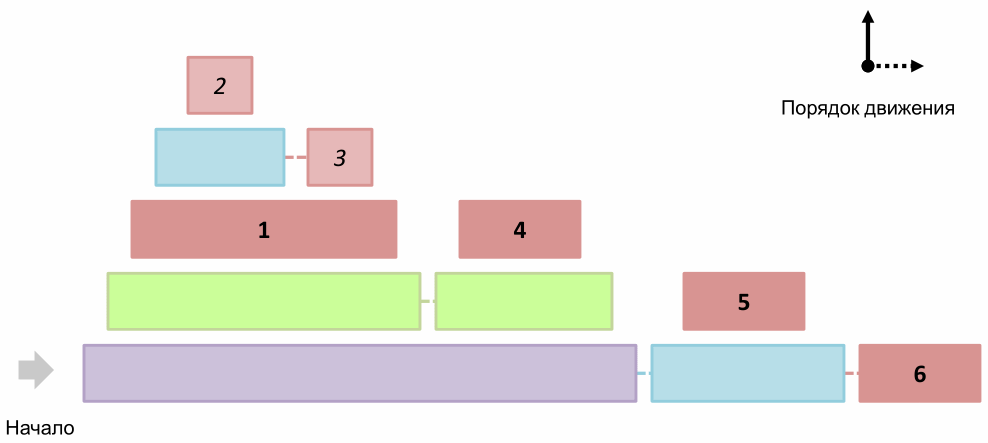
\includegraphics[width=3.2in]{modifier_level_b}
	\caption{Пример применения модификатора <<level>>.}
	\label{fig:modifier_level_b}
\end{figure}

В дополнение к этому, для каждой R-функции, содержащей модификатор, ренерируется вспомогательная <<стартовая>> функция, принимающая рассматриваемый уровнем выше узел и проводящая инициализацию переменной-счетчика для реализаций модификаторов, подобных <<all>> и <<level>>.

***

Помимо модификаторов, R-функции способны осуществлять фильтрацию узлов на основании данных, извлекаемых из соответствующих точек интереса, которые были указаны при описании синтаксической конструкций целевого языка в аннотации грамматики.
Фильтрация осуществляется посредством проверки соответствия данных, представленных в точке интереса и текстового шаблона, задаваемого пользователем при составлении правил инструментирования.

В листинге~\ref{rfunc-pattern-example} приведен пример фрагменета из пользовательского описания правил инструментирования, в котором демонстрируется использование модификаторов совместно с фильтрацией по шаблону.
В листинге~\ref{rfunc-pattern-example-src} приведен соответствующий исходный текст синтезированной основной R-функции.

***

%%%%%%%%%%%%%%%%%%%%%%%%%%%%%%%%%%%%%%%%
\subsection{Функции инструментирования}
%%%%%%%%%%%%%%%%%%%%%%%%%%%%%%%%%%%%%%%%

***

I-функции (англ. $instrument$) -- это TXL функции, специализированные по типу обрабатывамых узлов дерева разбора, предназначенные непосредственно для выполнения инструментирования в соответствии с указанными в аннотации шаблонами (поиска и замены) и алгоритмом работы.
В листинге~\ref{ifunc-example} приведен пример исходного текста I-функции.

\begin{lstlisting}[frame=single, language=TXL, label={ifunc-example}, caption={Пример I-функции}]
function print_usefull_message_to_the_log_instrummenter_before_uid12 kw_Class [class_declaration] kw_Method [method_declaration]
	replace $ [statement]
		__NODE__ [if_statement]
	deconstruct __NODE__
		'if '( Condition [condition] ') Statement [statement]
		OptElseClause [opt else_clause]
	import TXLinput [stringlit]
	construct STD_POINTCUT [id]	    'before
	construct STD_NODE [id]	        _ [typeof __NODE__]
	construct STD_FILE [stringlit]  _ [+ TXLinput]
	construct STD_RULE [id]         'print_usefull_message_to_the_log
	construct POI_METHOD_NAME [stringlit]
		_ [__POI_get___POI_METHOD_NAME kw_Method]
	construct POI_CLASS_NAME [stringlit]
		_ [__POI_get___POI_CLASS_NAME kw_Class]
	construct msg [stringlit]
		_ [+ STD_POINTCUT] [+ " <"] [+ STD_NODE] [+ "> block in ["] [+ POI_CLASS_NAME] [+ "] class, in {"] [+ POI_METHOD_NAME] [+ "} method"]
	by
		'{
      'iLogger.log(Level.FINE, msg ');
      'if '( Condition ') '{ Statement '}
      OptElseClause
    '}
end function
\end{lstlisting}

***

%%%%%%%%%%%%%%%%%%%%%%%%%%%%%%%%%%%%%%%%
\subsection{Вспомогательные TXL функции}
%%%%%%%%%%%%%%%%%%%%%%%%%%%%%%%%%%%%%%%%

***

%%%%%%%%%%%%%%%%%%%
\subsubsection{H-функции}
%%%%%%%%%%%%%%%%%%%

***

H-функции (англ. $help$) -- это TXL функции, специализированные по типам обрабатывамых узлов дерева разбора, предназначенные для проверки принадлежности определенному контексту по передаваемым параметрам.

В листинге~\ref{hfunc-example} приведен пример H-функций с именами \lstinline{__belongs_to_context___namespace_m} и \lstinline{__not__belongs_to_context___namespace_m}.
Функция \lstinline{__belongs_to_context___namespace_m}, как видно из ее названия, реализует проверку принадлежности некоторого узла дерева разбора, который содержит данные с типом \lstinline{procedure_impl_decl} .

\begin{lstlisting}[frame=single, language=TXL, label={hfunc-example}, caption={Пример H-функции}]
function __belongs_to_context___namespace_m kw_Method [procedure_impl_decl]
	match [any]
		_ [any]
	construct __VOID__ [any]
		% void
	construct POI_METHOD_NAMESPACE_str [stringlit]
		_ [__POI_get___POI_METHOD_NAMESPACE kw_Method]
	where
		__VOID__ [__std__equal POI_METHOD_NAMESPACE_str "Main."]
end function


function __not__belongs_to_context___namespace_m kw_Method [procedure_impl_decl]
	match [any]
		_ [any]
	construct __VOID__ [any]
		% void
	where not
		__VOID__ [__belongs_to_context___namespace_m kw_Method]
end function
\end{lstlisting}

***

%%%%%%%%%%%%%%%%%%%
\subsubsection{G-функции}
%%%%%%%%%%%%%%%%%%%

***

G-функции (англ. $get$) -- это TXL функции, специализированные по типу обрабатывамых узлов дерева разбора, предназначенные для получения узлов, содержащих полезные значения, из промежуточных узлов дерева разбора, имеющих TXL тип, который описывает какую-либо важную синтаксическую конструкцию целевого языка программирования.

В листинге~\ref{gfunc-example} приведен пример G-функции.

\begin{lstlisting}[frame=single, language=TXL, label={gfunc-example}, caption={Пример G-функции}]
function __POI_get___POI_METHOD_NAME_FULL kw_Method [procedure_impl_decl]
	replace [stringlit]
		_ [stringlit]
	deconstruct kw_Method
		    ProcedureIntfDecl0 [procedure_intf_decl] _ [nested_decl_block] _ [procedure_body_semi]
	deconstruct ProcedureIntfDecl0
		    ProcedureSignature1 [procedure_signature] _ [repeat semi_directive] _ [opt ';]
	deconstruct ProcedureSignature1
		    _ [opt 'class] _ [procedure_keyword] ProcedureId2 [opt procedure_id] _ [opt formal_parameters] _ [opt colon_type]
	construct ProcedureId2_str [stringlit]
		_ [quote ProcedureId2]
	by
		ProcedureId2_str
end function
\end{lstlisting}

***

%%%%%%%%%%%%%%%%%%%
\subsubsection{W-функции}
%%%%%%%%%%%%%%%%%%%

***

W-функции (англ. $wrap$) -- это TXL функции, предназначенные для приведения стандартных операторов языка TXL, предназначенных для сравнения и поиска, и выполняемых над текстовыми/строковыми ($stringlit$ в текущей реализации прототипа) данными, из вида <<$A~[op~B]$>> (где $A$ -- имя некоторой переменной, $B$ -- значение или имя некоторой другой переменной, $op$ -- оператор сравнения), в котором один аргумент является основным аргументом функции-оператора сравнения, а второй -- второстепенным, в вид <<$[op~A~B]$>>, что удобно при объединении операций сравнения в форму КНФ или ДНФ при выполнении проверок по нескольким критериям одновременно.
\nomenclature{КНФ}{коньюнктивная нормальная форма}
\nomenclature{ДНФ}{дизъюнктивная нормальная форма}

В листинге~\ref{wfunc-example} приведен пример исходного текста W-функции с именем \lstinline{__std__lower_equal}, которая используется для реализации обертки над операцией \textit{меньше или равно}.

\begin{lstlisting}[frame=single, language=TXL, label={wfunc-example}, caption={Пример W-функции}]
function __std__lower_equal A [stringlit] B [stringlit]
	match [any]
		_ [any]
	where
		A [<= B]
end function
\end{lstlisting}

***

Помимо стандартных операторов сравнения, таких как <<больше>>, <<меньше>>, <<равно>> и др., были реализованы следующие специальные опции:
\begin{itemize}[noitemsep]
  \item \textit{P has X} --
  текстовые данные, представленные в точке интереса $P$, сдержат в себе подстроку $X$. Текстовый фрагмент $X$ может как содержаться в начале, в середине и в конце проверяемого текста, так и повторяться неограниченное количество раз.

  \item \textit{P matches T} --
  текстовые данные, представленные в точке интереса $P$, соответствуют текстовому шаблону $T$. ***

  \item \textit{P exists} --
  явно указывает на необходимость существования в контексте инструментирования любых данных для выбранной точки интереса $P$, допустимых в соответствии с гамматикой языка программирования. Допустимым значением, относительно грамматики, может являться отсутствие значения, т.е. данные опциональны. Если отсутствие данных не помешает извлечь это опциональное значение, то в точке интереса $P$ будет содержаться пустая строка, иначе проверяемый узел дерева разбора будет удален из рассмотрения по причине несоответствия описываемому контексту. Использование этой опции не накладывает дополнительных ограничений на текстовое содержимое.
\end{itemize}

***

%%%%%%%%%%%%%%%%%%%%%%%%%%%%%%%%%%%%%%%%%%%%%%%%%%%%%%%%%%%%%%%%%%%%%%%%%%%%%%%%
\section{Выводы}
%%%%%%%%%%%%%%%%%%%%%%%%%%%%%%%%%%%%%%%%%%%%%%%%%%%%%%%%%%%%%%%%%%%%%%%%%%%%%%%%

В этом разделе были сформулированы задачи
***
